\documentclass[../../main.tex]{subfiles}

\graphicspath{{../../fig/}}
\setcounter{section}{0}

\begin{document}

\chapter{宇宙マイクロ波背景放射(CMB)偏光観測}
宇宙マイクロ波背景放射(Cosmic Microwave Background: CMB)とは、宇宙の創生から38万年後に物質から脱結合した光子のことであり、我々が観測できる最古の光である。
その発見はペンジアスとウィルソンによって1965年に行われ\cite{1965ApJ...142..419P}、
その後Cosmic Background Explorer(COBE)衛星により強度の周波数依存性(スペクトル)が測定された\cite{1996ApJ...473..576F}。
測定されたスペクトルは温度が$\SI{2.725}{K}$の黒体輻射のスペクトルと一致し(図\ref{fig:cobe})、
CMBの強度が天球面上の各点においてわずかな違いはあれど、ほとんど一様等方であることも確認された。
この事実はかつて宇宙が熱平衡状態にあったことを示し、宇宙が高温高密度の状態から膨張して現在に至るビッグバン宇宙モデルを支持する強力な証拠となった。
こうして現代の宇宙論の基礎を築き、発展させてきたCMBは、現在ではその偏光情報からインフレーション宇宙論の証拠を探ることができると期待されている。

本章では、はじめに現在の標準的な宇宙モデルである$\Lambda\mathrm{CDM}$モデルの概要と抱える問題について述べ、
次いでその問題の解決策としてインフレーション宇宙論について述べる。
その後、インフレーションがCMBパワースペクトルにどのような変化をもたらすかについて述べ、最後に本論文の構成について述べる。

\colortext{red}{最後の本章で〜の部分は最後に考える。}
\begin{figure}[H]
    \centering
    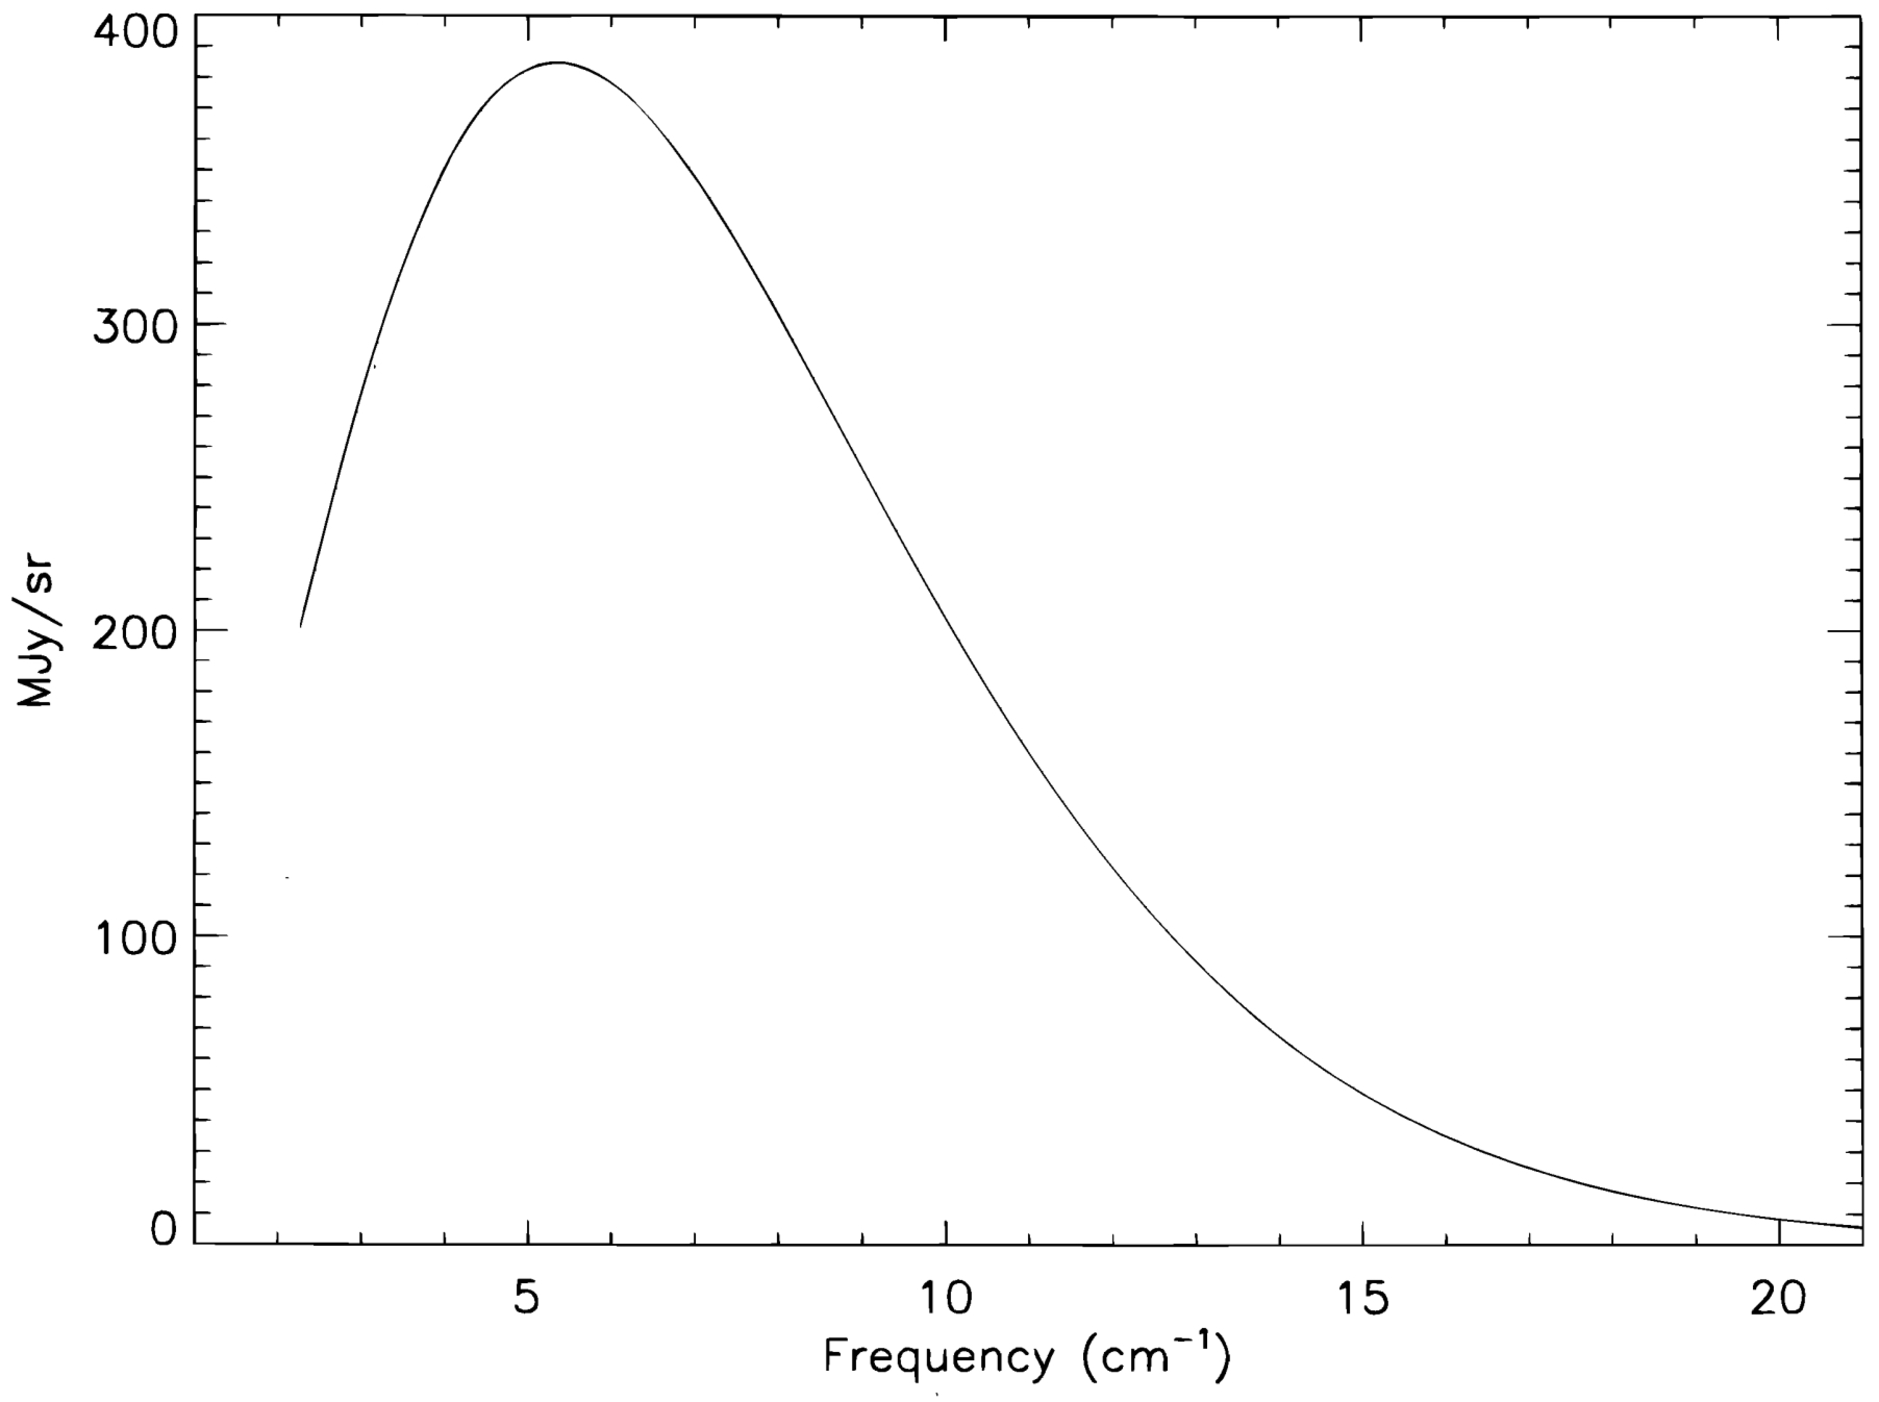
\includegraphics[width=0.6\textwidth]{intro/cobe.pdf}
    \caption{COBE衛星によるCMBのスペクトル測定値を黒体輻射のスペクトルでfittingした結果。}
    \label{fig:cobe}
\end{figure}

\section{$\Lambda\mathrm{CDM}$モデル}
現在の標準的な宇宙モデルである$\Lambda\mathrm{CDM}$モデルについて述べる。
まず、アインシュタイン方程式は、計量テンソル$g_{\mu\nu}$、アインシュタインテンソル$G_{\mu\nu}$とエネルギー運動量テンソル$T_{\mu\nu}$を用いて
\begin{equation}
    \label{eq:einstein}
    G_{\mu\nu}+\Lambda g_{\mu\nu}=8\pi GT_{\mu\nu}
\end{equation}
とかける。ここで、$G$は重力定数、$\Lambda$は宇宙定数である。また、自然単位系を採用した。
一様等方な宇宙では、その計量はフリードマン・ルメートル・ロバートソン・ウォーカー計量(以下、FLRW計量と呼ぶ)
\begin{equation}
    \label{eq:rwmetric}
    \dd{s}^2=-\dd{t}^2+a^2(t)\qty[\frac{\dd{r}^2}{1-Kr^2}+r^2\dd{\Omega}^2]
\end{equation}
で記述される。ここで、$a(t)$はスケールファクター、$K$は宇宙の曲率を表す。
また、宇宙の物質が完全流体であることを仮定すると、エネルギー運動量テンソルを
\begin{equation}
    \label{eq:emtensor}
    T_{\mu\nu}=\mqty(-\rho&0&0&0\\0&P&0&0\\0&0&P&0\\0&0&0&P)
\end{equation}
と表すことができる。ここで、$\rho$はエネルギー密度、$P$は圧力である。
エネルギー運動量テンソルを用いてエネルギー保存則を考えると
\begin{equation}
    \label{eq:energyconservation}
    \dot{\rho}+3\dfrac{\dot{a}}{a}(\rho+P)=0
\end{equation}
を得る。
式\eqref{eq:rwmetric}、式\eqref{eq:emtensor}を式\eqref{eq:einstein}に代入し、$(0,\,0)$に注目すると
\begin{align}
    \label{eq:friedmann}
    H^2:=\qty(\dfrac{\dot{a}}{a})^2 &= \dfrac{8\pi G}{3}\rho+\dfrac{\Lambda}{3}-\dfrac{K}{a^2}
\end{align}
を得る。これをフリードマン方程式と呼ぶ。$H:=\dot{a}/a$はハッブル定数である。
エネルギー密度$\rho$は、物質による寄与と放射による寄与とに大別することができる。
各々のエネルギー密度$\rho_m$、$\rho_r$はそれぞれ$a^{-3}$、$a^{-4}$に比例するため、フリードマン方程式は
\begin{equation}
    \label{eq:friedmann2}
    H^2=H_0^2\qty[\dfrac{\Omega_m}{a^3}+\dfrac{\Omega_r}{a^4}+\dfrac{\Omega_{K}}{a^2}+\Omega_{\Lambda}]
\end{equation}
と書ける。
ここで、$H_0$は現在のハッブル定数、$\Omega_m,\,\Omega_r,\,\Omega_{K},\,\Omega_{\Lambda}$はそれぞれ物質、放射、曲率、宇宙定数の密度パラメータであり
% 現在の各成分のエネルギー密度$\rho_{m,\,0},\,\rho_{r,\,0}$を用いて
\begin{align}
    \label{eq:omega}
    \Omega_m&:=\dfrac{8\pi G\rho_{m}}{3H_0^2},\quad
    \Omega_r:=\dfrac{8\pi G\rho_{r}}{3H_0^2},\quad
    \Omega_{K}:=\dfrac{-K}{H_0^2a^2},\quad
    \Omega_{\Lambda}:=\dfrac{\Lambda}{3H_0^2}
\end{align}
と表される。これらの密度パラメータは
\begin{equation}
    \label{eq:omegaconstraint}
    \Omega_{m}+\Omega_{r}+\Omega_{\Lambda}+\Omega_{K}=1
\end{equation}
を満たすが、これまでのCMBの観測は$\Omega_{m}+\Omega_{r}+\Omega_{\Lambda}=1$という結果を示しているため、宇宙は平坦であると考えられている\cite{Bennett_2003}。


$\Lambda\mathrm{CDM}$モデルには、以下の3つの問題をもつ。
\begin{enumerate}
    \item 地平線問題:CMBの温度揺らぎは天球面上のどの方向を見ても$\Delta T/T\sim 10^{-5}$と非常に小さい。
    これは因果関係を持たないはずの2点の温度が高い精度で一致していることを意味しており、$\Lambda\mathrm{CDM}$モデルはこの理由を説明できない。
    \item 平坦性問題:これまでの観測によれば、現在の宇宙は曲率がほとんどゼロである。宇宙の曲率の密度パラメータ$\Omega_{K}$は、時間発展とともに成長するため、
    宇宙初期に遡ると$\Omega_{K}$は不自然なほどに小さくなければならない。
    \item モノポール問題:大統一理論などの素粒子標準理論を超えた理論は、しばしば宇宙初期に磁気モノポールが生成されることを予言する。
    しかし、現在にいたるまで磁気モノポールは発見されていない。
\end{enumerate}
\section{インフレーションモデル}
前節にて述べた3つの問題の解決策として有力視されている理論が、
宇宙初期において宇宙が指数関数的に膨張したとするインフレーションモデルである。
この急激な膨張は因果律を持つ領域を急激に拡大し、空間を平坦にし、モノポールの濃度を薄めることで
地平線問題、平坦性問題、モノポール問題を解決することができる。

インフレーションモデルは佐藤、グースらによって1981年に提唱された\cite{10.1093/mnras/195.3.467}\cite{PhysRevD.23.347}が、
現在では多種多様なバリエーションを有する\cite{Tsujikawa_book}。
ここでは、宇宙初期にインフラトンというスカラー場$\phi$によって引き起こされ、
スローロール近似を課したインフレーションについて紹介する。

一様等方な宇宙のもとでのインフラトンの運動方程式は
\begin{equation}
    \label{eq:EoM_infraton}
    \ddot{\phi}+3H\dot{\phi}+c^2\pdv{V}{\phi} = 0
\end{equation}
と与えられる。$H$はハッブル定数である。
また、曲率$K=0$のフリードマン方程式\eqref{eq:friedmann}はインフラトンのエネルギー密度の寄与が主要であるとすると
\begin{equation}
    \label{eq:friedmann_infraton}
    3H^2M_{\mathrm{pl}}^2 = \dfrac{1}{2c^2}\dot{\phi}^2 +V(\phi)
\end{equation}
となる。$M_{\mathrm{pl}}=\sqrt{1/8\pi G}$は換算プランク質量である。
ここで、スローロール近似と呼ばれる、インフレーションが十分長い時間続くための近似
\begin{align}
    \qty|\dfrac{\dot{\phi}^2}{V(\phi)}| \ll 1,\qquad \qty|\dfrac{\ddot{\phi}}{H\dot{\phi}}| \ll 1
\end{align}
を課す。式\eqref{eq:EoM_infraton}と\eqref{eq:friedmann_infraton}から
\begin{align}
    H^2 &= \dfrac{V(\phi)}{3M_{\mathrm{pl}}} \\
    \dot{H} &= -\dfrac{\dot{\phi}}{2c^2M_{\mathrm{pl}}^2}
\end{align}
を得る。以上から、インフレーション中のスケール因子$a$は
\begin{align}
    a&\propto e^{\mathcal{N}} \\
    \mathcal{N} &:= -\int_{t_f}^{t}H\dd{\tilde{t}} = -\dfrac{1}{M_{\mathrm{pl}}^2}\int_{\phi_f}^{\phi}\dfrac{V}{\partial V/\partial \phi}\dd{\tilde{\phi}}
\end{align}
のように指数関数的に増大していく。ここで、$t$はインフレーション中の時刻、$t_f$はインフレーションが終わる時刻であり、
$\phi_f$はインフレーションが終わる時刻での$\phi$である。
$\mathcal{N}$はe-folding数と呼ばれ、典型的に$50<\mathcal{N}<60$程度だと考えられている。

インフレーションにおけるスケール因子の指数関数的増加は空間の指数関数的膨張を引き起こす。
また、この膨張に伴い、時空の量子揺らぎを古典的なスケールに引き延ばす。
具体的には、FLRW計量\eqref{eq:rwmetric}をデカルト座標系で書き直した上で
\begin{equation}
    \label{eq:jikuuyugami}
    \dd{s}^2 = -\qty(1+2\Phi)\dd{t}^2 + a^2\qty(1-2\Psi)\qty(\delta_{ij}+h_{ij})\dd{x_i}\dd{x_j}
\end{equation}
といった揺らぎを与える。
ここで、$\Phi$は重力ポテンシャル、$\Psi$は曲率揺らぎ、$h_{ij}$はテンソル揺らぎを表し、いずれも微少量である。
$h_{ij}$は重力波として見なすことができ、$z$軸正の方向に進む重力波は
\begin{equation}
    h_{ij} = \mqty(h_{+} & h_{\times} & 0\\
                   h_{\times} & h_{+} & 0\\
                   0 & 0 & 0
                   )
\end{equation}
と2つの基本モード($+$モードと$\times$モード)を用いて表すことができる。
図\ref{fig:gravitational_wave}に$+$モードと$\times$モードが作る空間の歪みを示す。
\begin{figure}[H]
    \centering
    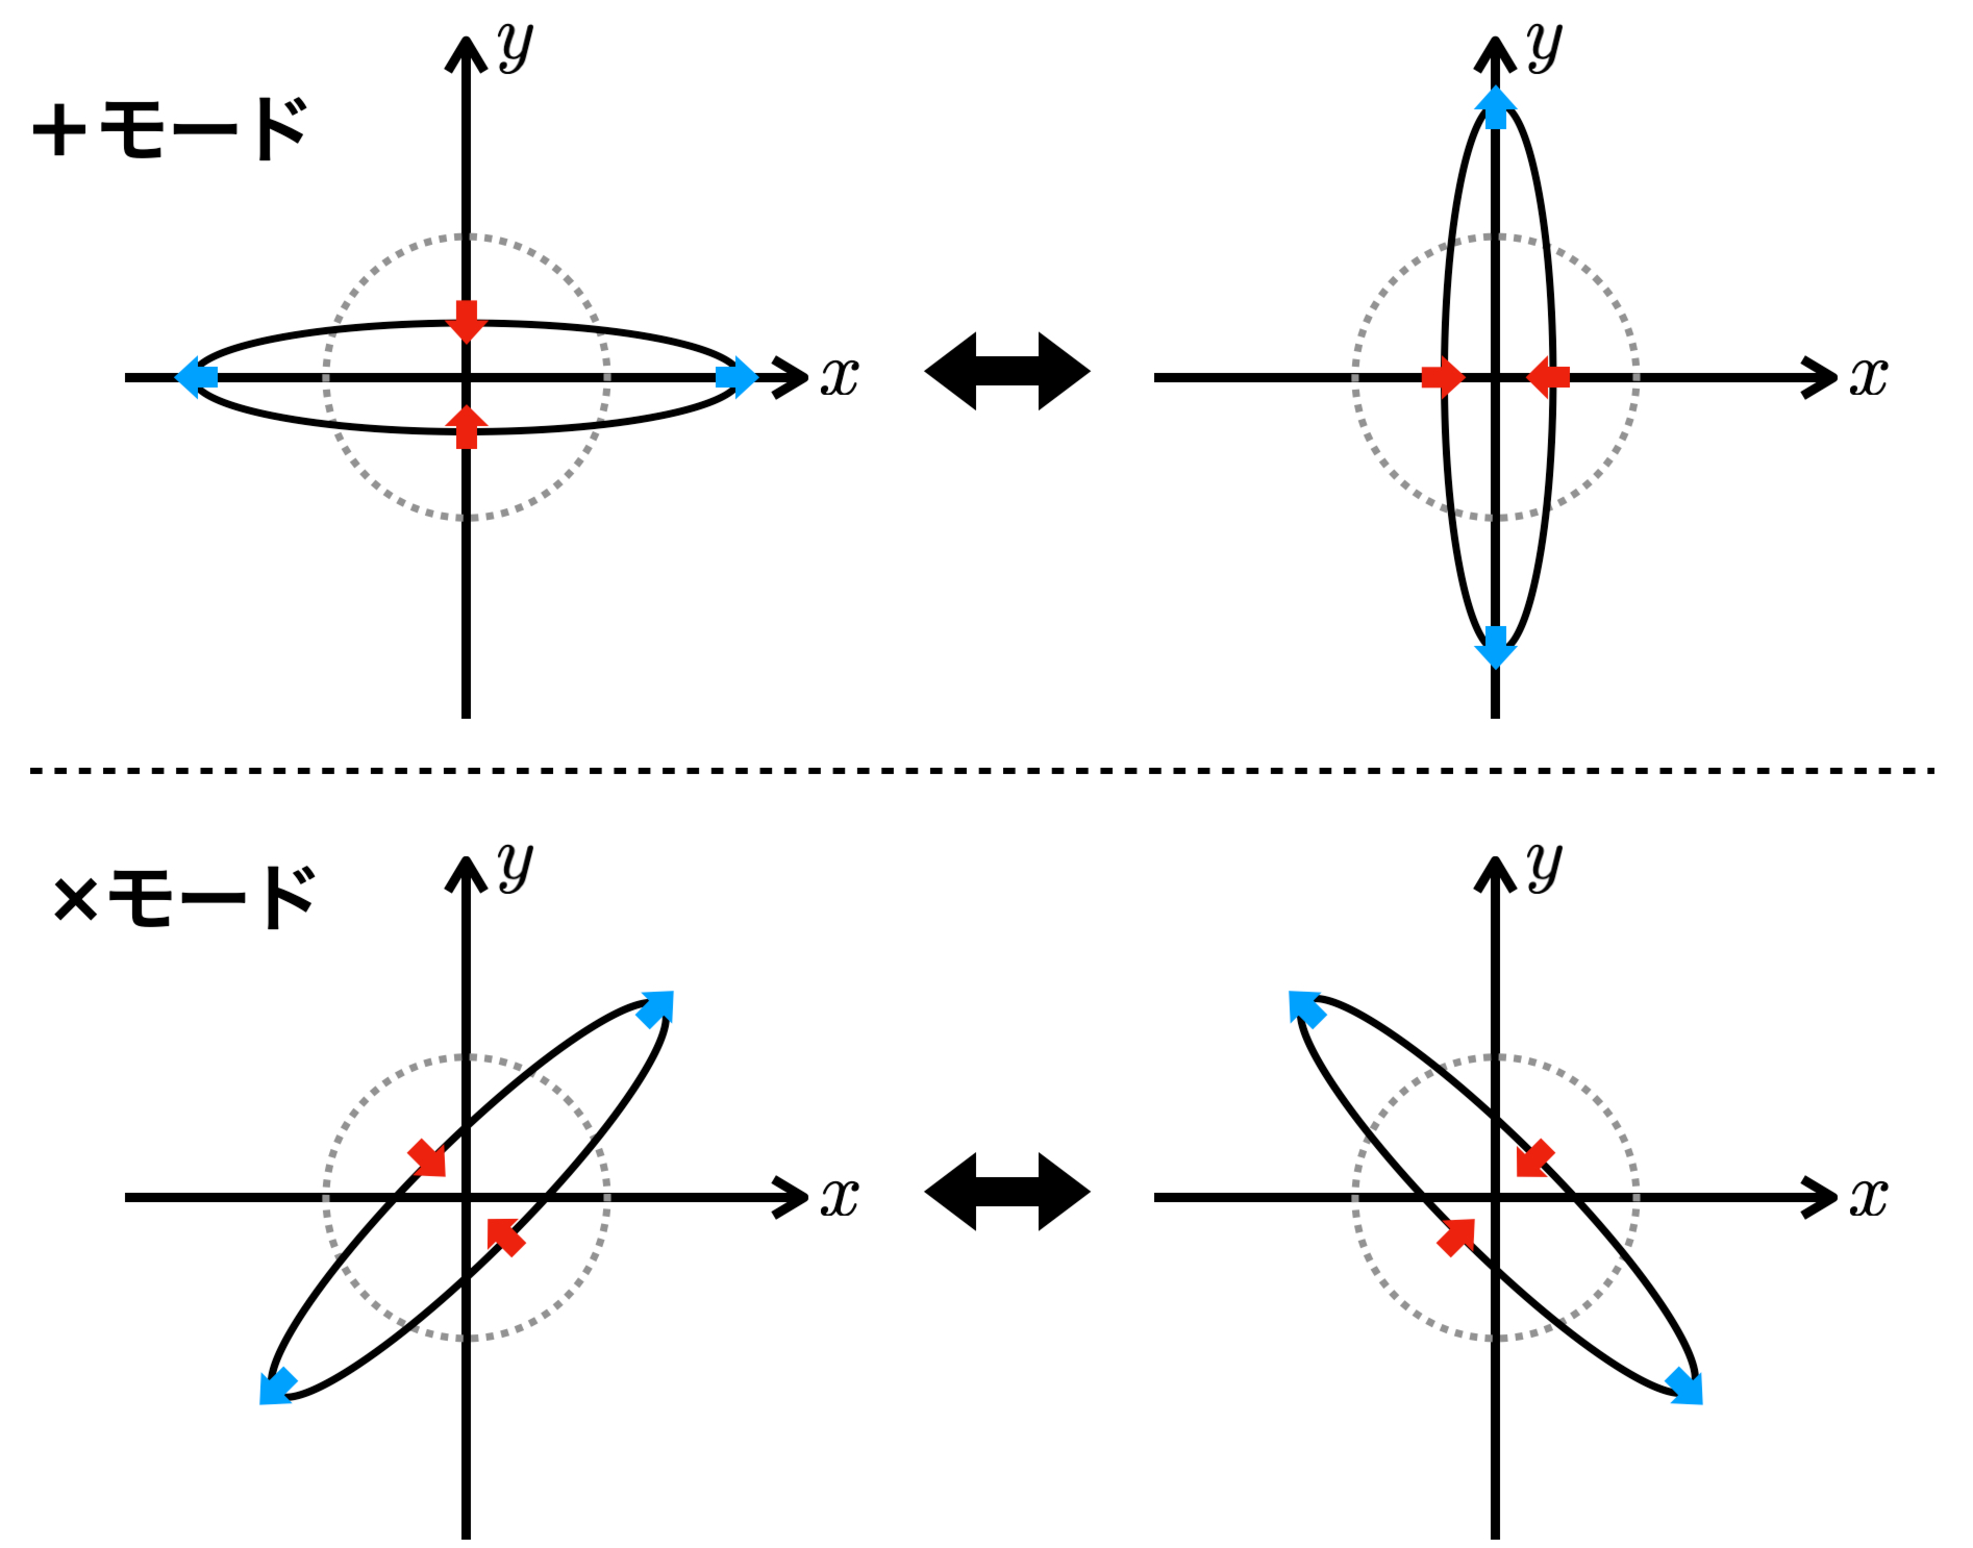
\includegraphics[width=0.8\textwidth]{intro/gravitational_wave.pdf}
    \caption{重力波の$+$モード(上)と$\times$モード(下)が作る空間の歪み。
    歪みのない時空上での円(点線)が、時空が歪むことで伸び縮みされ楕円(実線)になっている。}
    \label{fig:gravitational_wave}
\end{figure}

\section{CMBの温度異方性と偏光}
インフレーションによって生じた時空の歪みは、CMBの温度に異方性を作る\cite{1967ApJ...147...73S}。
式\eqref{eq:jikuuyugami}中の$\Phi,\,\Psi$はスカラー揺らぎと呼ばれる温度の揺らぎを、$h_{ij}$はテンソル揺らぎと呼ばれる温度の揺らぎを作る。
CMBの偏光にEモードと呼ばれる偏光パターンを、
Bモードと呼ばれる特有の偏光パターンを生む。
% 式\eqref{eq:jikuuyugami}中の$\Phi,\,\Psi$はスカラー揺らぎと呼ばれ、CMBの偏光にEモードと呼ばれる偏光パターンを、
% $h_{ij}$はテンソル揺らぎと呼ばれ、Bモードと呼ばれる特有の偏光パターンを生む。
本節では、はじめにCMBの温度異方性をどのように定式化するか述べ、過去の観測実験による結果を述べる。
その後、温度異方性がどのような偏光パターンを生むかについて述べる。

\colortext{red}{スカラー揺らぎを音波の疎密波のように表されることを述べるか?}
\subsection{CMBの温度異方性とパワースペクトル}
天球面上の各点におけるCMBの温度$T$に対して、温度揺らぎを$\Delta T = T-\bar{T}$と定義する。
$\bar{T}$は平均温度である。この温度揺らぎ$\Delta T$を、球面調和関数$Y_{\ell m}$で展開すると
\begin{equation}
    \Delta T = \sum_{\ell=1}^{\infty}\sum_{m=-\ell}^{\ell}a^{T}_{\ell m}Y_{\ell m}
\end{equation}
となる。この展開係数$a^{T}_{\ell m}$を用いて、に渡ってCMBパワースペクトル$C^{TT}_{\ell}$を
\begin{equation}
    C^{TT}_{\ell} = \dfrac{1}{2\ell+1}\sum_{m=-\ell}^{\ell}\qty(a^{T}_{\ell m})^{*}a^{T}_{\ell m}
\end{equation}
と書く。これは座標系によらないという点で優れた統計量となっている。
また、$\ell$は天球を見込む立体角$\Delta \Omega$と対応づいており、おおよそ$\Delta\Omega \simeq 180\tcdegree/\ell$と結びつく。

図\ref{fig:planck_cmb}にPlanck衛星によって観測されたCMBの温度異方性の全天マップを示す。
また、図\ref{fig:planck_powerspectrum}に同じくPlanck衛星によって得られたパワースペクトルを示す\cite{Planck_2020}。
\begin{figure}[H]
    \centering
    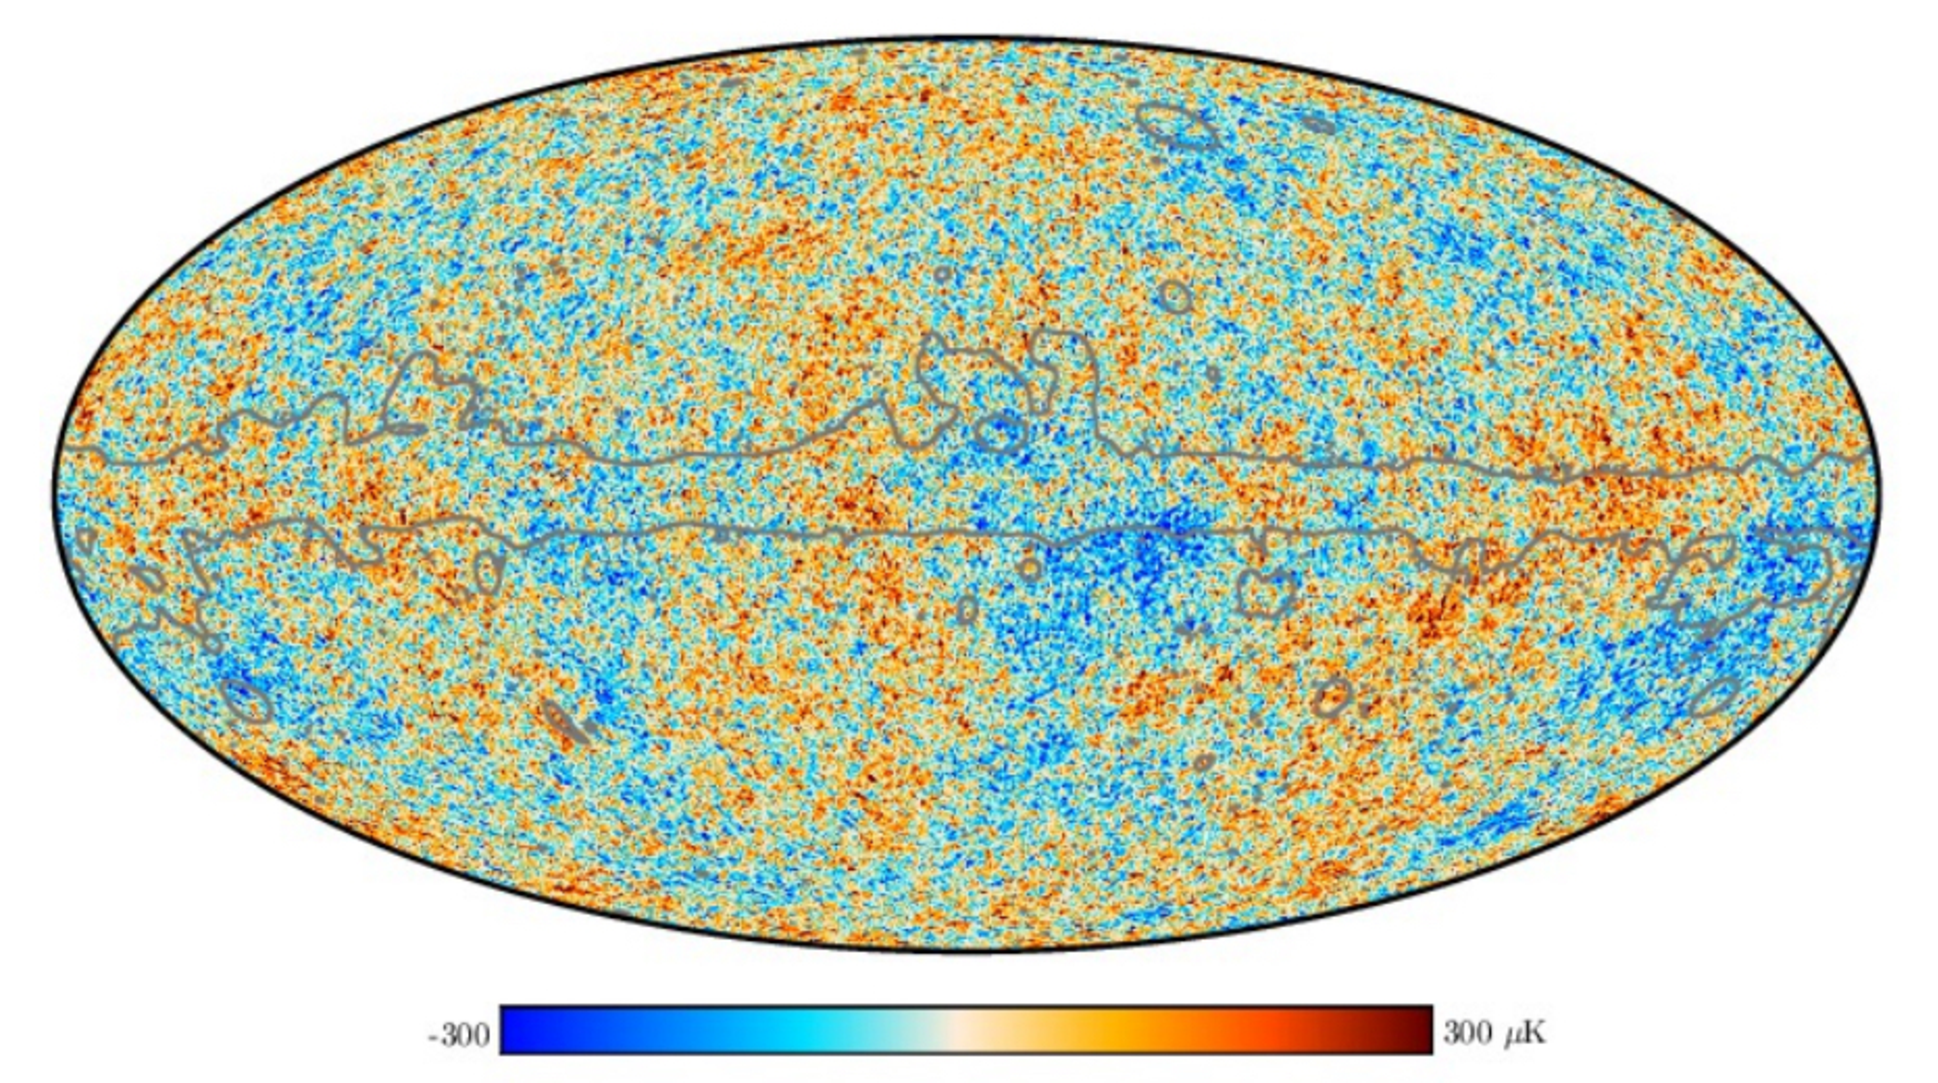
\includegraphics[width=0.8\textwidth]{intro/planck_cmb.pdf}
    \caption{Planck衛星によって得られた温度異方性の全天マップをモルワイデ図法で描いたもの\cite{Planck_2020}。
    色の分布は平均温度との差を表しており、赤色が平均よりも高温な部分、青色が平均よりも低温な部分を表す。}
    \label{fig:planck_cmb}
\end{figure}
\begin{figure}[H]
    \centering
    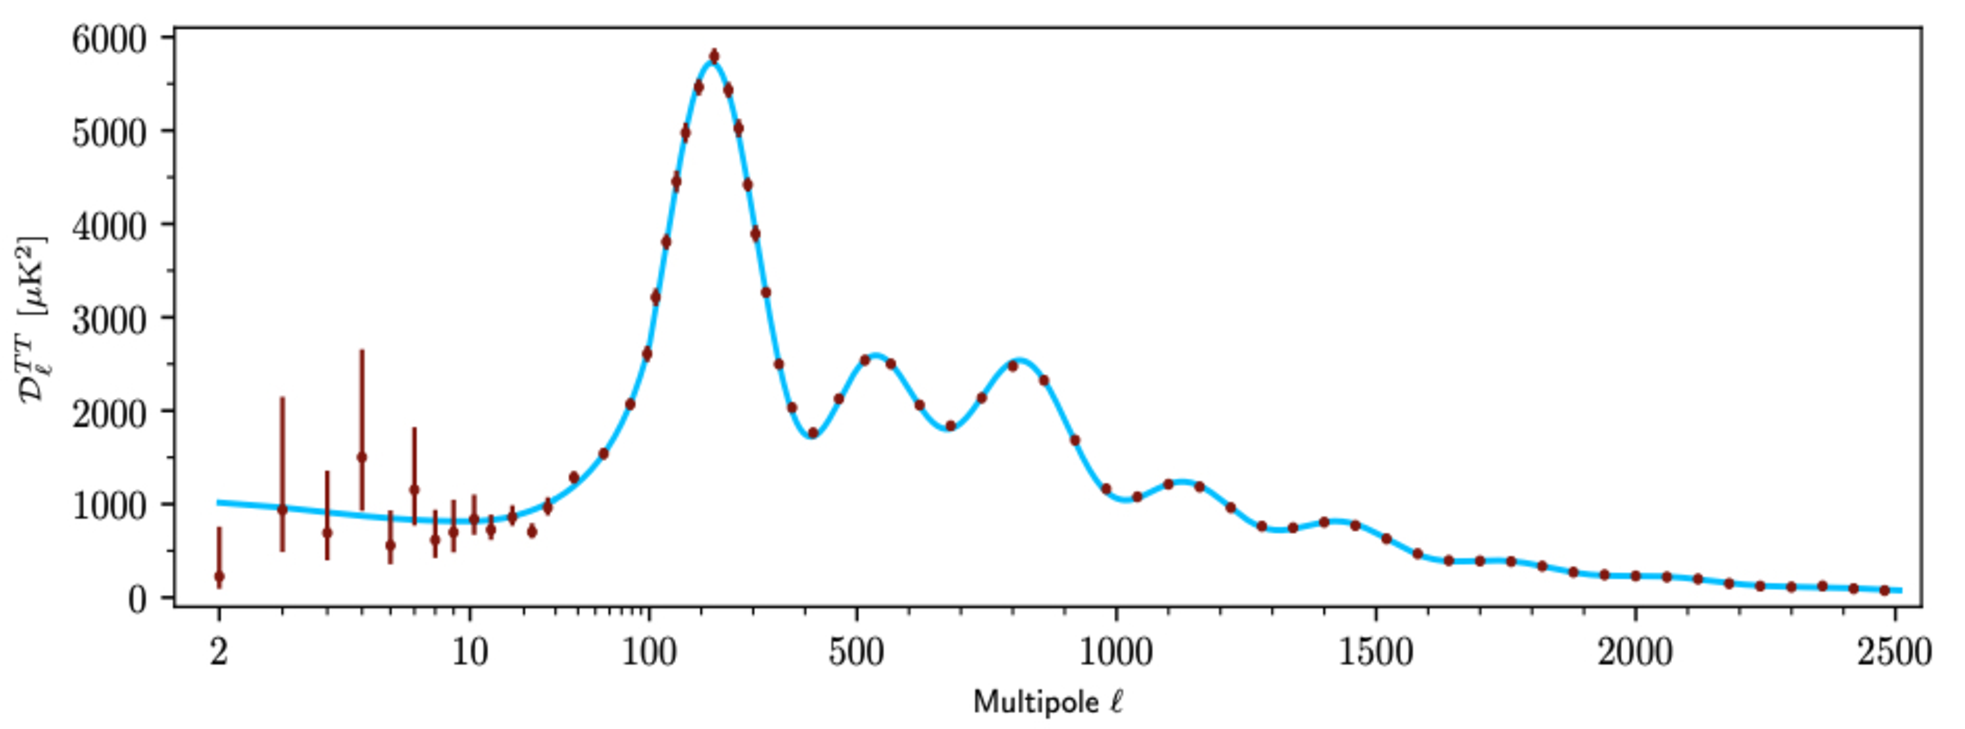
\includegraphics[width=0.8\textwidth]{intro/planck_powerspectrum.pdf}
    \caption{Planck衛星によって得られたパワースペクトル\cite{Planck_2020}。
    横軸に$\ell$、縦軸は\\$D^{TT}_{\ell}=\ell(\ell+1)C^{TT}_{\ell}/2\pi$を示している。}
    \label{fig:planck_powerspectrum}
\end{figure}
\subsection{四重極温度異方性による偏光の生成}
四重極温度異方性はトムソン散乱の散乱角の異方性と相まってCMBに偏光を生じさせる。
図\ref{fig:thomson_polarization}に四重極温度異方性を持つ空間と、トムソン散乱による偏光の生成メカニズムを示す。
最終散乱面上に$xy$平面にとり、最終散乱面から観測者に向かって$z$軸をとる。
$xy$平面上には$x$軸上に高温領域が、$y$軸上に低温領域があるような四重極の温度異方性があるとする。
このとき、$xy$平面上の原点にある電子は、周囲からやってくる光をトムソン散乱にしたがって観測者に向かって散乱する。
トムソン散乱により観測者が偏光として観測できるのは、もともと$xy$平面上に偏光方向を持っていた光の成分のみであり、
高温領域の光は低温領域よりも強度が高いため、観測者が見る偏光方向は低温領域を繋げたような直線偏光となる。
\begin{figure}[H]
    \centering
    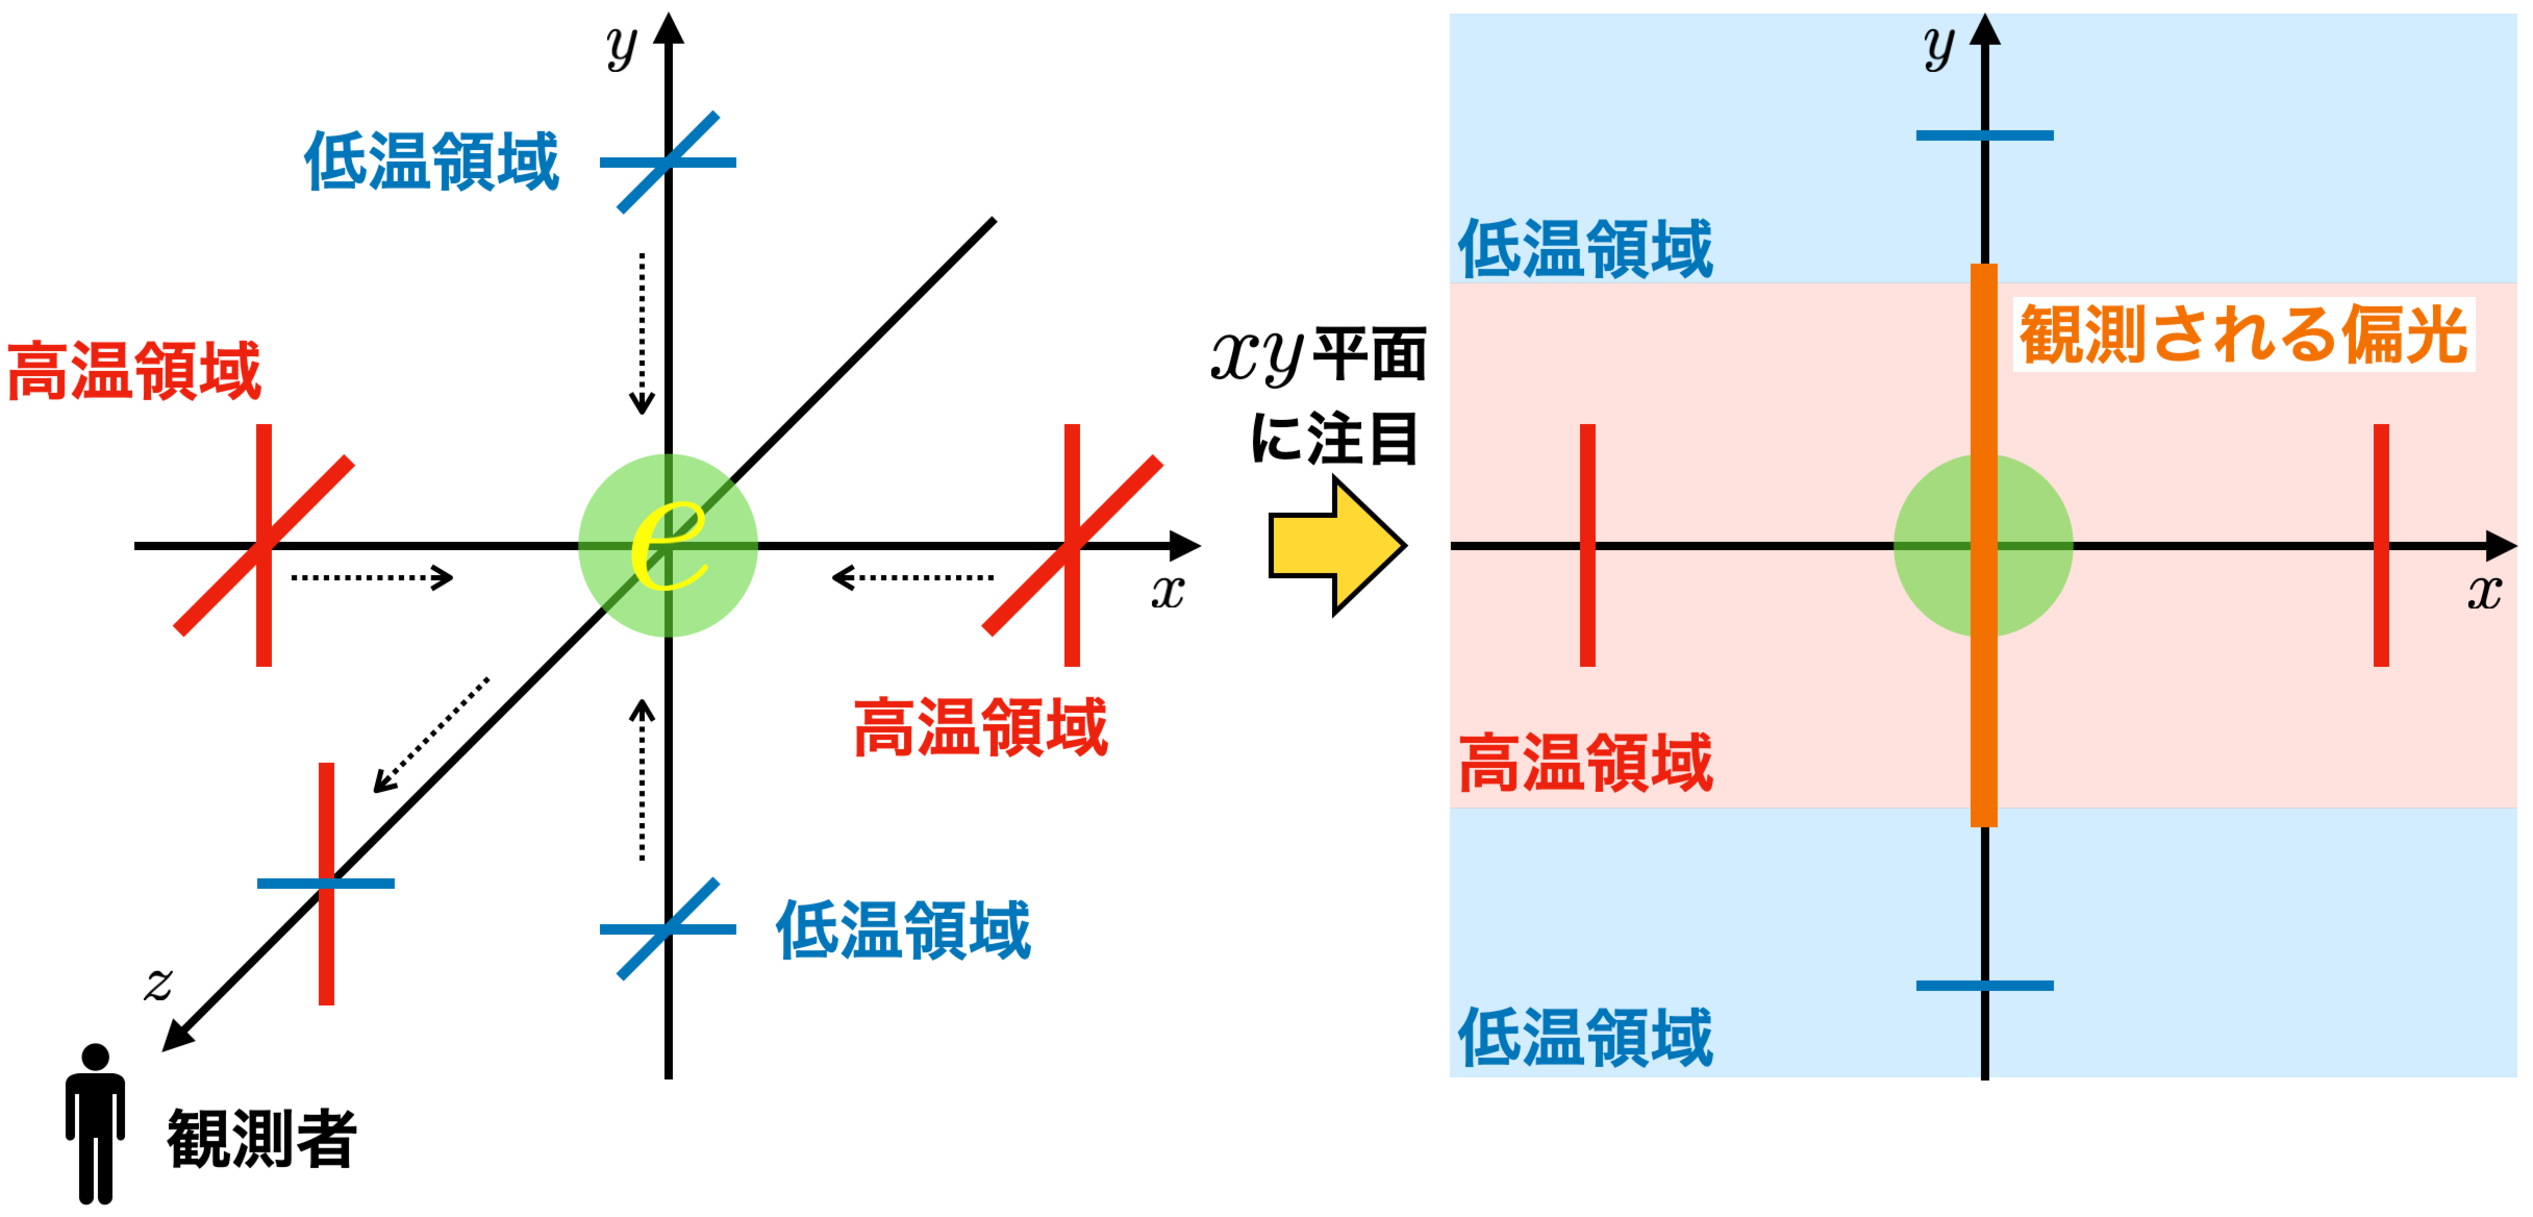
\includegraphics[width=1.0\textwidth]{intro/thomson_polarization.pdf}
    \caption{(左)四重極に分布する高温領域と低温領域からくる光が電子によってトムソン散乱され観測者に届く様子。
    赤色、青色の直線はそれぞれ高温領域からやってくる光と、低温領域からやってくる光の直線偏光方向を示す。
    (右)観測者から見た$xy$平面の様子。橙色で描いた線が観測者が見る直線偏光である。}
    \label{fig:thomson_polarization}
\end{figure}

\subsection{スカラー揺らぎが作る偏光パターン}
スカラー揺らぎは音波のような疎密波として伝わっていると理解される。

\section{本論文の構成}

\end{document}